
\documentclass{article}

\usepackage{graphicx}
\usepackage[usenames,dvipsnames,svgnames,table]{xcolor}
\usepackage[utf8]{inputenc}
\usepackage[T1]{fontenc}
\usepackage{titlesec}
\usepackage{cite}
\usepackage{hyperref}
\usepackage{amsmath}
\usepackage{mathtools}
\usepackage{multirow}
\usepackage{tabularx}  % for 'tabularx' environment and 'X' column type
\usepackage{ragged2e}  % for '\RaggedRight' macro (allows hyphenation)
\newcolumntype{Y}{>{\RaggedRight\arraybackslash}X}
\usepackage{booktabs}  % for \toprule, \midrule, and \bottomrule macros
\usepackage{pifont}
\usepackage{enumitem}
%\usepackage{bera}
\usepackage{xcolor}
\usepackage{listings}

\setlist{parsep=0pt,listparindent=\parindent}

\newcommand{\sectionbreak}{\clearpage}

%%% JSON LISTING

\colorlet{JSONPUNCTCOLOR}{red!60!black}
\definecolor{JSONBACKGROUNDCOLOR}{HTML}{EEEEEE}
\definecolor{JSONDELIMCOLOR}{RGB}{20,105,176}
\colorlet{JSONNUMBERCOLOR}{magenta!60!black}

\lstdefinelanguage{json}{
    captionpos=b,
    basicstyle=\normalfont\ttfamily\small,
    %numbers=left,
    %numberstyle=\scriptsize,
    %stepnumber=1,
    %numbersep=8pt,
    showstringspaces=false,
    breaklines=true,
    frame=single,
    backgroundcolor=\color{JSONBACKGROUNDCOLOR},
    literate=
     *{0}{{{\color{JSONNUMBERCOLOR}0}}}{1}
      {1}{{{\color{JSONNUMBERCOLOR}1}}}{1}
      {2}{{{\color{JSONNUMBERCOLOR}2}}}{1}
      {3}{{{\color{JSONNUMBERCOLOR}3}}}{1}
      {4}{{{\color{JSONNUMBERCOLOR}4}}}{1}
      {5}{{{\color{JSONNUMBERCOLOR}5}}}{1}
      {6}{{{\color{JSONNUMBERCOLOR}6}}}{1}
      {7}{{{\color{JSONNUMBERCOLOR}7}}}{1}
      {8}{{{\color{JSONNUMBERCOLOR}8}}}{1}
      {9}{{{\color{JSONNUMBERCOLOR}9}}}{1}
      {:}{{{\color{JSONPUNCTCOLOR}{:}}}}{1}
      {,}{{{\color{JSONPUNCTCOLOR}{,}}}}{1}
      {\{}{{{\color{JSONDELIMCOLOR}{\{}}}}{1}
      {\}}{{{\color{JSONDELIMCOLOR}{\}}}}}{1}
      {[}{{{\color{JSONDELIMCOLOR}{[}}}}{1}
      {]}{{{\color{JSONDELIMCOLOR}{]}}}}{1},
}

%%% RUTA LISTING

\definecolor{RUTABACKGROUNDCOLOR}{HTML}{EEEEEE}

\lstdefinelanguage{ruta}{
    captionpos=b,
    basicstyle=\normalfont\ttfamily\small,
    %numbers=left,
    %numberstyle=\scriptsize,
    %stepnumber=1,
    %numbersep=8pt,
    showstringspaces=false,
    breaklines=true,
    frame=single,
    backgroundcolor=\color{RUTABACKGROUNDCOLOR},
}

%%%
% Commands

\newcommand{\ID}[1]{{\textsc{#1}}}
\newcommand{\PATH}[1]{\mbox{\texttt{#1}}}

\newcommand{\TODO}[1]{\texttt{\textcolor{YellowOrange}{(#1)}}} % for inline TODO
\newcommand{\REST}[1]{\textsf{#1}}

\newcommand{\tablewidth}{0.9\linewidth}
\newcommand{\VERTICALTEXT}[1]{\rotatebox{90}{#1}}
\newcommand{\MULTIROW}[2]{\multirow{#1}{*}{\vbox{#2}}}

\newcommand{\CMARK}{\ding{51}} % check mark
\newcommand{\XMARK}{\ding{55}} % cross mark

\newcommand{\ONEBC}{\ding{182}} % 1 in a black circle
\newcommand{\TWOBC}{\ding{183}} % 2 in a black circle

\newcommand{\ONEWC}{\ding{192}} % 1 in a white circle
\newcommand{\TWOWC}{\ding{193}} % 2 in a white circle

\newcommand{\UNDERBRACE}[2]{\underbrace{\text{#1}}_{\mathclap{\text{#2}}}}

%
%%%

\title{Large-scale Information Extraction from Neuroscientific Literature}

\date{Spring 2015}

\author{Marco Antognini}

\begin{document}

\maketitle

\begin{center}
    Master Semester Project under the supervision of\\
    Jean-Cédric Chappelier \& Renaud Richardet\\
    Artificial Intelligence Laboratory LIA - EPFL
\end{center}

\begin{abstract}
  \TODO{todo}
\end{abstract}

\pagenumbering{gobble}
\newpage
\pagenumbering{arabic}


\tableofcontents

\section{Introduction}

The neuroscientists at the Blue Brain Project~\cite{bbp}, in their quest to model the human brain,
have to understand the interactions between the different components of the brain such as cells or
brain regions and connect their effects with other parts of the brain or other organs.  However,
since the amount of information is colossal and is obviously not memorisable by individual human
being or even by a team of researchers, tools need to be created in order to extract the relevant
data from the scientific literature in a precise and fast manner.

Sherlok~\cite{sherlok} was created to solve this large-scale text mining problem. Based on a
Representational State Transfer (REST) API, Sherlok is a service capable of extracting information
relevant to specific situation directly from a given text. It is designed to be both user- and
developer-friendly and flexible so that it can analyse text via standard REST requests.

Currently, the main dependency of Sherlok is, but is not restricted to, bluima~\cite{bluima}, which
is an open source project developed at the Blue Brain Project and consists of a large collection of
UIMA-based \emph{annotators}~\cite{uima} (also called \emph{engines} -- both terms are used
interchangeably) that generate metadata from the input text. We will focus on those specific
annotators for this project.

Generated metadata consists of a collection of \emph{annotations}. Each annotation has a begin and
end position in the raw text, a type identifier and in some cases extra attributes. It ranges from
tags as simple as sentences boundaries to more complex notions such as brain regions.

For example, annotating the following sentence for brain regions, generates the following
annotations (for simplification, part of speech (PoS) tags are not shown here). Additionally,
Sherlok reports brain regions \ONEWC\; and \TWOWC\; as a co-occurrence.

\begin{align*}
    & \text{Substantial numbers of tyrosine hydroxylase-immunoreactive cells in}\\
    & \text{the } \UNDERBRACE{dorsal raphe nucleus}{Brain Region \ONEWC}
      \text{ were found to project to the } \UNDERBRACE{nucleus accumbens}{Brain Region \TWOWC}
      \text{.}
\end{align*}

While each annotator works on its own to generate metadata, Sherlok lets the user combines them in
\emph{pipelines} where the output of one engine is used as the input for the next one. And in order
to reuse engines in different pipelines, Sherlok separates their definitions: engines are first
grouped in bundles, which make the bridge between Sherlok's scripting system and the UIMA annotators
written in Java so that they can be used by several pipelines.

In addition to basic configuration parameters such as arbitrary strings or integers, the algorithms
used in the different engines can rely on external resources which can be as simple as a file
containing a list of countries, but could also consist of large trained models (e.g. to detect part
of speech) or directories of configuration files. The main goal of this project was to decouple
those algorithms from their resources in bluima in order to add flexibility to the installation,
update and usage of those resources in Sherlok.

Initially, bluima relied on a system-wide setting to locate its resources. However, since we wanted
to make Sherlok run on as many systems as possible -- which should include a server architecture
where a dedicated machine is in charge of storage -- we couldn't rely on this property any longer.
Hence, the first and main task of this project was to devise a system capable of working without
hard coded paths.

This project was threefold:

\begin{itemize}[label=\ding{228}]
    \item the first and main task was to devise a system capable of working without hard coded
        paths;
    \item a second task was the design of a clever system for installing and loading resources on
        demand (i.e. when loading a pipeline);
    \item the third and final task was to port a full brain regions NER and connections pipeline
        from bluima to Sherlok, which includes sentence detection, part of speech tagging, species
        recognition, measures and units extraction and more~\cite{bluima_2013}.
\end{itemize}

\TODO{include quick plan of paper}

\section{Sherlok}

Sherlok is an open source service for text information extraction created at the Blue Brain Project
to extend and popularise bluima engines. However, Sherlok is not restricted to neuroscience and as
such, does not require any prior neuroscientific knowledge.

\subsection{REST-Based Service}

The service provided through a classic Representational State Transfer (REST) API can be installed
in-house by system administrators to match the specific needs of researchers. From the user
perspective, only a basic understanding of the Hypertext Transfer Protocol (HTTP) is required to
build queries used to communicate with Sherlok.

%\begin{table}[h]
    %\centering
    %\begin{tabularx}{1.2\linewidth}{l l >{\hsize=2cm}X Y}
                %&       & \MULTIROW{2}{Additional Parameters}   &           \\
        %Method  & Path  &                                       & Action    \\

        %\toprule

        %GET  & \REST{/annotate/<pipeline>}      & text          &
            %\MULTIROW{2}{Annotates the given text with the selected pipeline (the pipeline version is
            %optional).} \\
             %&                                  & version (opt) &  \\
        %\\ \\ % fix v-spacing

        %\midrule

        %POST & \REST{/annotate/<pipeline>}      & text          &
            %\MULTIROW{2}{Like the previous one, but the text (and the optional pipeline version) is
            %posted in JSON format.} \\
             %&                                  & version (opt) &  \\
        %\\ \\ % fix v-spacing

        %\midrule

        %GET  & \REST{/pipelines}                &               &
            %\MULTIROW{1}{Lists the installed pipelines.} \\
        %% \\ % fix y-spacing

        %\midrule

        %GET  & \multicolumn{2}{ l }{\REST{/pipelines/<pipeline>/<version>}} &
            %\MULTIROW{1}{Downloads the given version of the mentioned pipeline definition.}  \\
        %\\ \\ % fix y-spacing

        %\midrule

        %POST & \REST{/pipeline}                 &               &
            %\MULTIROW{1}{Install the pipeline definition present in the body of the request} \\
        %\\ \\ % fix y-spacing

        %\midrule

        %DELETE & \REST{/pipeline/<pipeline>/<version>}  &       &
            %\MULTIROW{1}{Uninstall the given version of the mentioned pipeline} \\
        %\\ % fix y-spacing

        %\midrule

        %POST & \REST{/test}                     & pipeline      &
            %\MULTIROW{1}{Runs the tests of the (temporary) pipeline defined in the body of the request.} \\
        %\\ \\ % fix y-spacing

        %\midrule

        %GET  & \REST{/test/<pipeline>}          & version (opt) &
            %\MULTIROW{1}{Runs the tests for the given installed pipeline.} \\
        %\\ % fix y-spacing

        %\midrule

        %GET  & \REST{/reload}                   &               &
            %\MULTIROW{1}{Reloads Sherlok's settings.} \\
        %% \\ % fix y-spacing

        %\midrule

        %\bottomrule
    %\end{tabularx}
    %\caption{\TODO{caption me}}
    %\label{tab:sherlok_rest_api}
%\end{table}

%\TODO{add resources, cleaning and bundle requests}

%\TODO{actually, this table should be in the doc, not here. Here, just explain the main ones
%(annotate, test, install and remove)}

While its implementation is written in Java, any language or tool with basic socket support can
communicate with Sherlok and benefits from its capabilities without going through the frequent
required hassle to build wrappers to communicate between Java and another language. Additionally,
as a proof of concept, Sherlok provides a JavaScript, Java and Python client API to emit the
standard REST queries in those languages. And due to the nature of REST and HTTP protocols they can
easily be extended to support more languages.

From an end-user point of view, the HTTP request

\[
    \REST{GET /annotate/<pipeline>?text=<input>}
\]

is all there is to know to use a given pipeline to process some text: nothing is installed on the
user side; instead everything is directly available on Sherlok's server without investing in
powerful personal computers. And if the existing pipelines don't fit the user's needs a new pipeline
can be submitted to Sherlok which will automatically install the required dependencies, would they
be Java packages or regular files needed at runtime. Additionally, Sherlok comes with a basic web
editor to easily install new pipelines, edit them and process text without manually writing any REST
queries.

From a system administrator point of view, Sherlok is no less flexible or harder to use. The
installation procedure is as simple as extracting an archive and launching an executable. And
because Sherlok runs on the Java Virtual Machine (JVM), any system with a proper Java Runtime
Environment 7 (JRE7) is able to run Sherlok. The memory and disk requirement depends on the
pipelines that the users will run. However, the system administrator doesn't have to pay resources
for pipelines that are not used: Sherlok easily allows obsolete pipelines or resources to be
deleted.

Were one server not capable of providing enough computational power to handle all users' requests,
several instance of Sherlok can be run in a \emph{slave} mode to balance the workload on several
machines.

Moreover, if the system administrator wants to restrict the installation or modification of
pipelines, he can run Sherlok in \emph{sealed} mode to freeze the configuration of the service.
While Sherlok doesn't have any particular Access Control List (ACL) mechanism to support
fine-grained access control and restrict users permissions on a case by case basis, custom ACL
system can easily be built on top of Sherlok: a simple proxy program can integrate restricted access
using for example Unix accounts or a Lightweight Directory Access Protocol (LDAP) server to filter
requests before Sherlok can process them.

Figure \ref{fig:sherlok_basic_rest_call} depicts how a REST query is handled from a very high level
point of view by Sherlok.

\begin{figure}
    \centering
    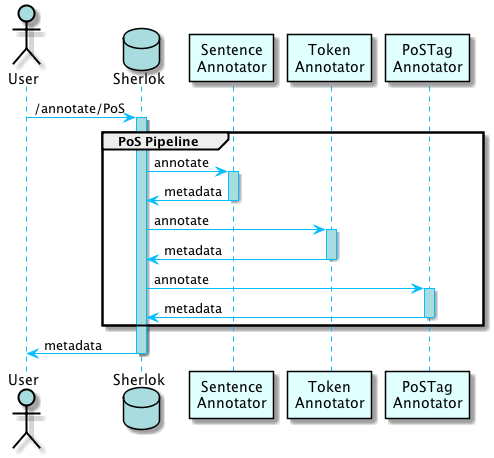
\includegraphics[width=0.7\linewidth]{res/sherlok_basic_rest_call.png}
    \caption{Part of Speech Pipeline}
    \label{fig:sherlok_basic_rest_call}
\end{figure}

\subsection{UIMA-Based Configurable Service}

Internally, Sherlok will process the input text through Unstructured Information Management
Architecture (UIMA)~\cite{uima} engines or more generally through a Rule-based Text Annotation
(RUTA) scripts~\cite{ruta}. Both RUTA and UIMA are projects of the Apache Software Foundation
\cite{apachefundation} focusing in analysing large volumes of unstructured information in order to
discover knowledge that is relevant to an end user. While Sherlok focuses on the Java Frameworks for
UIMA, it could be extended in the future to also support the C++ or Scaleout Frameworks.

In order to let users who are not Java developers combine engines together, Sherlok has a Java
agnostic configuration system that separate the definition of engines from their usage in pipelines.

\begin{description}
    \item[Bundles] The user lists the UIMA engines that he wants to use in \emph{bundles} by specifying
        the Java package dependencies, the required resource files and configure the different
        parameters of the engines. To simplify installing resources, Sherlok supports download at
        execution time of Git repositories or HTTP(S) URLs, but also lets the user specify local
        path on the server if needed.
    \item[Pipelines] The user writes the RUTA script which can be as simple as chaining engines from
        the bundles configuration files in \emph{pipelines}. The whole features set of RUTA is
        available to the user so that simple scripts don't require any Java implementation from the
        user. Similarly to bundles, Sherlok allow downloading resources for pipeline automatically.
\end{description}

By default Sherlok comes with pipelines to extract information about brain regions, part of speech
and much more. The engines used in those pipelines come from bluima, which is presented in Section
\ref{sec:bluima}.

The annotations produced by a pipeline are returned from the server in JSON format~\cite{json}. For
example, Listing \ref{lst:json_sententence_detection} highlights the annotations in JSON format
produced by the \ID{bluima.sentence} pipeline when processing ``\textit{Terminologies which lack
semantic connectivity hamper the effective search in biomedical fact databases and document
retrieval systems. We here focus on the integration of two such isolated resources, the term lists
from the protein fact database UNIPROT and the indexing vocabulary MESH from the bibliographic
database MEDLINE.}''

In this listing are displayed three annotations: one \ID{DocumentAnnotation}, which provides insight
on the language of the processed document, and two \ID{Sentence}, each of which have a general
\ID{componentId} representing which NLP component has been used to derive the annotation.
Additionally, all three annotations have information about the corresponding range of the text that
they cover.

% The following listing is too big to fit properly. Also there are so many things that are not
% really interesting for the reader.
%\begin{lstlisting}[language=json,firstnumber=1]
%{"_context" : {
    %"_types" : {
      %"DocumentAnnotation" : {"_id" : "uima.tcas.DocumentAnnotation",
        %"_feature_types" : {"sofa" : "_ref" } },
      %"Sentence" : {"_id" : "de.julielab.jules.types.Sentence",
        %"_feature_types" : {"sofa" : "_ref" } },
      %"Sofa" : {"_id" : "uima.cas.Sofa",
        %"_feature_types" : {"sofaArray" : "_ref" } },
      %"Annotation" : {"_id" : "uima.tcas.Annotation",
        %"_feature_types" : {"sofa" : "_ref" },
        %"_subtypes" : ["DocumentAnnotation",  "Annotation" ] },
      %"AnnotationBase" : {"_id" : "uima.cas.AnnotationBase",
        %"_feature_types" : {"sofa" : "_ref" },
        %"_subtypes" : ["Annotation" ] },
      %"TOP" : {"_id" : "uima.cas.TOP",
        %"_subtypes" : ["AnnotationBase",  "Sofa" ] },
      %"Annotation" : {"_id" : "de.julielab.jules.types.Annotation",
        %"_feature_types" : {"sofa" : "_ref" },
        %"_subtypes" : ["Sentence" ] } } },
  %"_views" : {
    %"_InitialView" : {
      %"DocumentAnnotation" : [
        %{"sofa" : 1,  "begin" : 0,  "end" : 328,  "language" : "en" } ],
      %"Sentence" : [
        %{"sofa" : 1,  "begin" : 0,  "end" : 135,  "componentId" : "de.julielab.types.OpenNLPSentenceDetector" },
        %{"sofa" : 1,  "begin" : 136,  "end" : 328,  "componentId" : "de.julielab.types.OpenNLPSentenceDetector" } ] } },
  %"_referenced_fss" : {
    %"1" : {"_type" : "Sofa",  "sofaNum" : 1,  "sofaID" : "_InitialView",  "mimeType" : "text",  "sofaString" : "Terminologies which lack semantic connectivity hamper the effective search in biomedical fact databases and document retrieval systems. We here focus on the integration of two such isolated resources, the term lists from the protein fact database UNIPROT and the indexing vocabulary MESH from the bibliographic database MEDLINE." } } ,
  %"_stats" : {
    %"_pipeline_resolution": 3285,
    %"_annotation": 435
  %}
%}
%\end{lstlisting}

\begin{lstlisting}[float,language=json,
                   caption=Excerpt of JSON output for sentence detection.,
                   label=lst:json_sententence_detection]
"DocumentAnnotation" : [
  { "begin" : 0,    "end" : 328,  "language" : "en" }
],
"Sentence" : [
  { "begin" : 0,    "end" : 135,
    "componentId" :
        "de.julielab.types.OpenNLPSentenceDetector" },
  { "begin" : 136,  "end" : 32
    "componentId" :
        "de.julielab.types.OpenNLPSentenceDetector" }
]
\end{lstlisting}

For quality purpose, Sherlok also allows the user to embed tests for pipelines that can be run
through the \REST{GET /test/<pipeline>} query in order to ensure that pipelines continue to work
properly after updating Sherlok or the engines' dependencies.

\section{Bluima, UIMA and RUTA}
\label{sec:bluima}

Bluima is an open-source collection of UIMA readers~\cite{uima} augmented by multiple engines
developed at the Blue Brain Project~\cite{bbp} to perform large-scale information extraction from
the neuroscientific literature. It includes for example a species annotator based on the Linnaeus
library~\cite{linnaeus}, or the OpenNLP toolkit~\cite{opennlp} to perform Part of Speech tagging,
sentence splitting and more. The complete list of subprojects is detailed in
Table~\ref{tab:bluima_subprojects}.

\begin{table}[h]
    \centering
    \begin{tabularx}{\tablewidth}{@{} l Y @{}} % no margin at extremum
        \toprule

        OpenNLP~\cite{opennlp} & a machine learning based toolkit for the processing of natural
        language text \\

        \midrule

        Linnaeus~\cite{linnaeus} & a general-purpose dictionary matching software, capable of
        processing multiple types of document formats in the biomedical domain \\

        \midrule

        & \TODO{add the others} \\

        \bottomrule
    \end{tabularx}
    \caption{bluima aggregated projects}
    \label{tab:bluima_subprojects}
\end{table}

UIMA-based applications are structured into components called \emph{analysis engines}, or
\emph{annotators}, which produce metadata in form of annotations. The implementation of such engines
can be either written in C++ or in Java, however C++ development seems rather marginal compared to
the amount of available libraries and tool for UIMA in Java, for which several implementation
strategies have been devised over the years. The most modern and popular API used to build
components is \emph{uimaFIT}~\cite{uimafit}: it aims to simplify the archaic XML description used in
earlier UIMA APIs to configure (C++ or Java) engines by writing both the implementation and
configuration of engines' parameters directly in Java. While Sherlok is compatible with any
UIMA-compatible technology, we focus on the uimaFIT approach in what follows.

At runtime, an annotator has mainly two actions: initialisation and processing. Annotations produced
by engines is stored in a Common Analysis System (CAS)~\cite{cas} general purpose data structure,
which allows the representation of objects with single-inheritance hierarchy, properties and values.
And in a pipeline of annotators, a single CAS instance is passed from one engine to the next so that
the data from previous engines can be used to filter data, augment existing annotations or produce
new ones.

Figure \ref{fig:pos_pipeline_uimafit} depicts how uimaFIT-based applications handle pipelines such
as PoS tagging: first, the text to be processed is loaded into a CAS instance, then engines are
created through uimaFIT factory system with the appropriate configuration settings and finally the
pipeline of engines is run.

\begin{figure}[h]
    \centering
    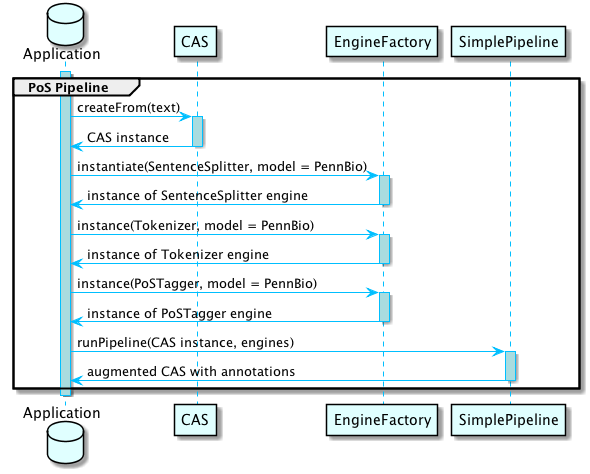
\includegraphics[width=0.9\linewidth]{res/uimafit.png}
    \caption{Part of Speech Tagging uimaFIT pipeline}
    \label{fig:pos_pipeline_uimafit}
\end{figure}

% TODO Doc
%These two tasks are modeled by implementing the \ID{initialize} and \ID{process}, respectively,
%methods of the Java interface \ID{AnalysisComponent}. +
%org.apache.uima.fit.component.JCasAnnotator_ImplBase

While uimaFIT is very convenient when writing an UIMA application that is entirely written in Java,
it becomes much more complex when we want to include a flexible external configuration as we do with
Sherlok. Moreover, and especially for simple pipelines, sometimes implementing a Java annotator
requires more boilerplate code than the actual algorithm.

To workaround this, an application can use the RUTA language~\cite{ruta}, which is an imperative
rule language extended with scripting elements that can also be used to define pipelines. To
illustrate this, Listing \ref{lst:ruta_example_dog} shows a very simple script that annotates
``dog'' as an ``Animal'' and Listing \ref{lst:ruta_example_pos} shows how RUTA can be used to run
the PoS pipeline from Figure \ref{fig:pos_pipeline_uimafit}. For this last example, unlike with
uimaFIT, the XML description of engines' parameters need to be available at runtime as it is not
embedded in the script itself.

\begin{lstlisting}[float,language=ruta,
                   caption=A basic RUTA script,
                   label=lst:ruta_example_dog]
DECLARE Animal;
W{REGEXP("dog") -> MARK(Animal)};
\end{lstlisting}

\begin{lstlisting}[float,language=ruta,
                   caption=PoS pipeline written in RUTA,
                   label=lst:ruta_example_pos]
ENGINE SentenceAnnotator;
ENGINE TokenAnnotator;
ENGINE PosTagAnnotator;

Document{-> EXEC(SentenceAnnotator)};
Document{-> EXEC(TokenAnnotator)};
Document{-> EXEC(PosTagAnnotator)};
\end{lstlisting}

Fortunately, uimaFIT provides tools to generate XML descriptions for classic engines so that we can
use RUTA to generate pipeline automatically for the user from a simpler description of the engines'
parameters than raw XML as follows:

\begin{enumerate}
    \item The user defines the engines with their parameters inside bundles;
    \item Then he defines the order of engines in a given pipeline;
    \item When the user wants to annotate a given text with the pipeline, Sherlok converts the
        engines, with their configured parameters, used by the pipeline into XML descriptions;
    \item Sherlok generates a RUTA script that uses the engine descriptions in the order of the
        pipeline;
    \item And finally, Sherlok runs the RUTA script and return the annotations back to the user.
\end{enumerate}

Additionally, Sherlok allows users to use the full RUTA language in pipelines to create even more
powerful tools. And in order to make configuration more flexible, as we will see in Section
\ref{sec:config_in_sherlok}, the user has the possibility to user configuration variables in bundles
or pipelines to download automatically remote resources.

\section{Packaging Strategy}

Initially all resources used by bluima's engines, such as models trained on the GENIA corpus
\cite{genia} to tag part of speech elements, were accessed via a system wide path variable. In this
section we will discuss the adopted strategy to improve this system and make bluima path agnostic in
order to improve its integration in Sherlok. In the Appendix \TODO{?} we show a few other alternatives
that were also considered during this project.

\subsection{Initial Situation}

Both bluima and Sherlok build system are based on Apache Maven~\cite{maven}, which allows developers
to define how a Java project should be compiled, packaged, tested and much more. One important
feature of Maven is its ability to download dependencies from centralised repositories where
developers can publish their releases. At the beginning of this project, however, bluima was not yet
available in Maven central which meant that to use it one had to clone its git repository, compile
and install it.

Yet, publishing bluima to Maven Central would not suffice to solve a bigger issue. Bluima widely
uses resource files in its engines and therefore needs to access those files at runtime. Originally,
it used a system global variable (\ID{BLUIMA\_HOME}) as many popular tools do nowadays (e.g. Java
with its \ID{JAVA\_HOME}) to locate specific files. Thus, using Maven to download and install Java
archives (jar) is not enough to locate those files later at runtime: the variable must be set at a
system-wide level by the user itself.

This made it clear that we needed a better engines-resources model or the integration of bluima in
Sherlok would imply that system administrators would have to manually install and configure bluima,
which in itself would defeat the whole purpose of Sherlok to make users' life better and automate
dependencies installation.

\subsection{Proposed Solutions}

There exist, as always, many methods to address this issue. But for this project, in addition to
ease the integration of bluima in other tools, we wanted to keep the refactoring and maintenance
cost low, allow resources to refer to one-another, make it possible to group files together in
\emph{batches}, avoid runtime performance penalties wherever possible and remove as little
flexibility from the users as possible.

\TODO{add § for runtime safety}

\subsubsection{Refactoring and Maintenance}

The first idea that we explored was to package resources inside jar archive and use Maven to
distribute them similarly to what DKpro~\cite{dkpro} does but in a less complex manner for the
users.

In a nutshell, packaging resources within jar archives has two important drawbacks. Firstly,
updating a resource file implies repackaging and redeploying the new version to, for example, Maven
Central, which can be quite a burden. One could argue that this is an administrative task that is
not frequent and therefore not significantly enough to discard this strategy. However, the second
issue is of much more concern.

As detailed in the Appendix \TODO{?}, this packaging strategy implies more refactoring than it seems
at first sight: in order to be able to use an engine with different resources (e.g. one might prefer
to use a probabilistic tokenizer trained on the GENIA corpus to process some inputs, but use a model
trained on a different corpus for some other inputs) and not hardcode them, we need a \emph{proxy}
to select from an identifier the appropriate files at runtime.

In the appendix we illustrate this with a technique using as the identifier the name of the class
that ``owns'' the desired resource file. Although the fact that the implementation of the proxy we
designed is based on the Java Reflection API is not related to the amount of refactoring needed to
adapt bluima to this packaging design, it significantly adds some complexity to the overall software
and therefore will increase its maintenance cost.

The Java API to access jar content is based on read-only access because, among other things, those
archives can be signed and thus modifying their content would threaten the integrity of the
signature or corrupt the archive.

The core refactoring issue with this design is that instead of working with \ID{File} objects or
paths as the initial implementation of bluima engines does, we would have to use \ID{InputStream} in
order to access the resources files because of how Java jar system was designed. And this can be
really problematic for some annotators. For example, the \ID{LinnaeusAnnotator}, which wraps the
external Linnaeus library~\cite{linnaeus}, uses an \ID{ArgParser} internally that cannot be created
from a data stream but absolutely requires a path to a configuration file.

Of course, some workarounds could be elaborated, such as copying the content of the file in the jar
archive to a temporary file and then use this file's path, but only on a case by case basis and that
those would most probably induce performance penalties.

\subsubsection{Resource Interdependency}

The \ID{LinnaeusAnnotator} also illustrate another feature that engines might need: the ability to
reference a resource file from another resource file via relative paths. With DKpro-like solutions,
the usage of stream to read resources content makes it much harder to allow such behaviour.

Workarounds for this specific issue usually imply modifying the engines and their underlying
implementation to work differently. In the case of \ID{Linnaeus\-Annotator} this would have meant to
completely rewrite the Linnaeus library since it is a closed-source utility, which is clearly out of
the scope of this three-month project.

\subsubsection{Batch Of Files}

Like with \ID{LinnaeusAnnotator}, the \ID{BrainRegionPipes} use a batch of files: a collection of
configuration files used together to set up an annotator or its dependencies. For the
\ID{BrainRegionPipes} the problem is easier since no file makes a reference to another one.
Nevertheless, it would be very verbose and painful to denote each and every of the ~30 files one by
one in the configuration of the engine. Hence, considering a batch of files simply as a collection
of files without a specific naming structure is not optimal. Depending on whether or not we base the
resource packaging system on a system similar to DKpro, the consequences differ:

\begin{itemize}

    \item Were we to use a packaging strategy based on jar files, we could introduce an arbitrary
        naming structure for the identifiers used to access the actual resource through the proxy
        system and have an \emph{aggregator proxy} that generates multiple data streams to each and
        every individual resources from a single root identifier. While this solution seems simple
        on the paper it actually requires as much refactoring as using one identifier by resource.

        Additionally, it doesn't solve the interdependency between resources as illustrated above
        with \ID{LinnaeusAnnotator}.

    \item If we apply the idea of names having an arbitrary but constant structure to the filenames
        directly instead of the identifiers used by a proxy, we can group the resource files
        together in an archive (e.g. a zip file) that would get extracted at runtime into a
        temporary directory.

        With this approach we have at least two significant advantages over the jar-based design
        without sub-archives. Firstly, it only requires a minimal refactoring of the current Java
        code to extract and use the data as the implementation is based on \ID{File}s or
        \ID{String}s representing paths. Secondly, it allows files to refer to one another through
        relative paths.

        However, this would imply adding a relatively complex version checking system in bluima
        and/or Sherlok: in order to not extract data from an archive when it is already available to
        prevent degrading performance too much, we would have to check if the data was already
        extracted and if that's the case that it is actually correct. This can be quite complex
        when, for example, upgrading resources. And this is without mentioning having several
        pipelines using the same engine but with different version of its resources, nor dealing
        with multiple concurrent annotation instances. Finally, if we take the example of Sherlok
        running on several servers, we introduce an issue of data accessibility and replication for
        cache purposes.

\end{itemize}

\subsubsection{Flexibility}

With all the different issues listed above, the jar-based packaging design seems rather inconvenient
to use, mainly because it involves a lot of refactoring. Moreover it adds some complexity to the
implementation. Some engines behave differently depending on the file type of some of their
resources: for example, the \ID{SuffixSensitiveGISModelReader} utility read the content of its input
resource differently depending if the file extension is ``.bin'' or ``.txt''. When using
\ID{InputStream} instead of \ID{File} the extension is lost and therefore need to be tracked with an
additional parameter.

In addition to all the above issues, we could argue that we actually remove flexibility from the
user by forcing him to use a Java system to archive and manage resources despite the fact that the
system using bluima could be Java agnostic from the final user point of view. It could actually be
quite painful for someone who is using a Source Control Management (SCM) tool, such as Git, to
manage two distinct files structures: one that is convenient to the user and one for our jar
archiving system.

Moreover, if we take the example of batch of files, at the end of the day, we have extracted some
data that the user had to package initially in order to make the installation process easy but
incredibly complexify the implementation.


\subsubsection{Adopted Solution}

We argue that the installation process for runtime resources could be much simpler than packaging
resources into jar files in the first place, potentially aggregating batch of files together in
sub-archives, then accessing those files via a proxy and an extra layer of resource identifiers,
potentially extracting sub-archives into a temporary directory, and by this mean forcing the user to
use a specific versioning system as DKpro-like systems do.

From bluima perspective, the user could simply installed the configuration files in a directory of
his choosing and configured the engines with paths to the actual resources without using any
system-wide variable. Withal, since this simpler approach does not enforce any versioning mechanism
at all, the user is free to implement any system that matches his needs. Following from this fact,
Sherlok can add an extra layer, directly integrated in the bundle \& pipeline configuration files, to
manage resources easily for the end users. Such system can, but is not restricted to, be based on
Git: a user can define a (batch of) resource(s) by a Git repository and an optional tag or commit
SHA and Sherlok then can automatically download and install the specific version of the resources.

This last solution allies the flexibility of using Java \ID{File} objects, and therefore involves
only little refactoring of bluima annotators, with the power of external, well-establish and
powerful SCM tools in addition to avoid the limitation of having to rely solely on \ID{InputStream}
to access resources. This is why it was selected and implemented in this project.

\begin{table}[h]
    \centering
    \begin{tabular}{l c c c c c}
        Strategy & \VERTICALTEXT{Refactoring-Friendly}
                 & \VERTICALTEXT{DRY-code}
                 & \VERTICALTEXT{Flexibility}
                 & \VERTICALTEXT{Repackaging Cost}
                 & \VERTICALTEXT{Runtime Safety} \\

        \toprule

        DKpro-Like~\cite{dkpro} & \XMARK & \CMARK & (\CMARK) & \XMARK & \XMARK \\

        \midrule

        Proxy-Based A & \XMARK & \CMARK & \XMARK & \XMARK & \CMARK \\

        \midrule

        Proxy-Based B & \XMARK & \CMARK & \XMARK & \CMARK & (\CMARK) \\

        \midrule

        Proxy-Based C & \XMARK & \XMARK & \XMARK & \XMARK & \CMARK \\

        \midrule

        Proxy-Based D & \XMARK & \CMARK & \XMARK & \CMARK & \XMARK \\

        \midrule

        Adopted Solution & \CMARK & \CMARK \CMARK & \CMARK \CMARK & \CMARK & \XMARK \\

        \bottomrule
    \end{tabular}
    \caption{Packaging Strategies Comparison}
    \label{tab:packaging_strategies}
\end{table}

\TODO{add explanation about the table and reference to index for the ``Proxy-Based''}

\subsection{Impact on bluima}

\TODO{minor refactoring}

\TODO{add path parameter for all files/directories}

\TODO{deprecated/remove code that still uses the global variable}

\TODO{how tests are impacted}

\TODO{Git submodules for resources for bluima}

\subsection{Configuration in Sherlok}
\label{sec:config_in_sherlok}

\TODO{where? -> pipeline + bundle (examples) + file structure}

\TODO{how? git/http/test + can easily be extended}

\TODO{where the data is saved and how it can be cleaned if needed}

\TODO{class diagram?}

\subsection{Possible Extensions}

\TODO{auto archive extractor / ssh / svn / hg / \dots}

\TODO{auto update for HTTP (using rfc + download if newer)}

\TODO{auto update for git branches (support for git hooks, \dots)}

\TODO{improve git download strategy (if SHA, depth 1, \dots)}

\section{Packaging: a first approach that didn't work}
\label{sec:packaging1}

\TODO{find better title}

The initial idea was to base the system on Apache Maven \TODO{ref}. However, while implementing the
strategy described below we realised that it was not as flexible as predicted. A better alternative
is presented in Section \TODO{ref{sec:packaging2}}. This section describes our first approach.

One of the first objective of this project was the disassociation of algorithms (engine annotators) and their different resources (model files, configuration files) and devise a packaging system, based on Apache Maven, that would be flexible while being simple and convenient to use and let the user define pipelines using specific annotators and models.

\subsection{Packaging}

\TODO{explain that packages would be released on public repo, and thus making them available}

\TODO{quickly present DKpro packaging strategy \& ant script. Say why we did not go with it.}

With Maven, main idea is to store a set of resources, such as dataset trained on a specific corpus of texts, in a jar file and access them in read-only mode at runtime. Package dependencies can be used to ensure that some files are available at runtime and ideally package version should be used to let the user update resources independently of the algorithms.

\TODO{Insert example, e.g. Sentence}

It might not be clearly apparent for someone not used to work with Java jar system, but with this approach we cannot modify the resource files at runtime since they have been packaged, and this for mainly two reasons. Firstly, the Java API doesn't provide standard tools to modify such archives. And secondly, if the jar archive were signed (which is the standard procedure) then modifying its content would actually break the signature and therefore corrupt the archive.

Additionally, the API to access resources inside jar files is not based on Java \ID{File} objects. Instead algorithms have to use \ID{InputStream} objects through \ID{ClassLoader} objects to access the content of a given file. We will discuss how the current code need to be refactored in Section \ref{sec:restructuring_bluima}.

Here we describe three alternatives that we used to contrast alternative strengths and weaknesses before concluding with a fourth variant that should match our needs. Below, \ID{ada} and \ID{bob} denote two variants of a kind of resource that are compatible with a common algorithm package, denoted \ID{algo}. The \ID{using*} packages can be thought as pipelines in the context of bluima/sherlok.

\subsubsection{Version A}

The first system we analysed spread each algorithm and set of resources into individual packages that depends on \ID{modeldep}, a proxy utility to access the resource files inside jar archives. If an algorithm depends on some resource file then it accepts as input parameter the model name (as a string) and uses the proxy to load the file. In this scenario pipeline packages have dependencies toward their annotators but also toward specific models as shown in Figure \ref{fig:pkgsysA}.

This system has several positive aspects. First of all, tests can be easily written by specifying potentially multiple resource packages as dependencies with Maven's test scope. Then, \ID{modeldep} also defines a clear Java interface to define the contract for models and their versions. Additionally, the proxy system centralises the utility to load resources and therefore eases maintenance by not involving code duplication in several packages. However, models could not be swapped on the fly since it would involve recompiling and repackaging \ID{using\_my\_algo}.  Alternatively, to prevent modifications, \ID{using\_my\_algo} could depend on both \ID{ada} and \ID{bob} packages but this would not be as flexible as we want it to be.

\begin{figure}
\centering
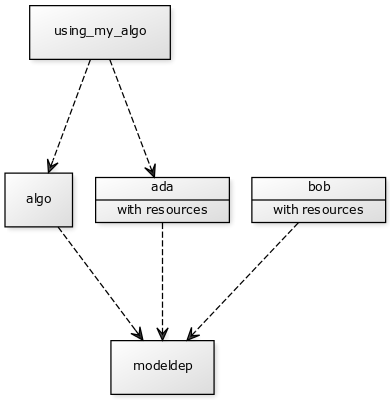
\includegraphics[width=200pt]{res/packaging_version_A.png}
\caption{Packaging Version A}
\label{fig:pkgsysA}
\end{figure}


\subsubsection{Version B}

The second approach is based on Maven's version string: an \ID{algo} will depend on an abstract \ID{model} which provide a mechanism to load a specific file from its jar archive and both \ID{ada} and \ID{bob} model versions are defined as subversion of \ID{model}. For example, the convention could be that if \ID{model} is defined as version \ID{0.1} then \ID{ada} will use the string \ID{0.1-ADA} to define its version and the \ID{algo} will accept versions in the range $ [0.1,0.2) $.

The model actually used will be either specified at compile time (cf. \ID{using.algo2}) or be selected at runtime depending on the installed packages (cf. \ID{using.algo1}) as depicted on Figure \ref{fig:pkgsysB}. While this offers a great flexibility to the user designing pipelines and allows him to swap models without repackaging anything, it means that test projects cannot ensure the correctness of more than one model version at a time. Moreover, if no specific version is bound to the pipeline, such as with \ID{using.algo1}, then there is no strong guarantee that a valid version is available at runtime.

\begin{figure}
\centering
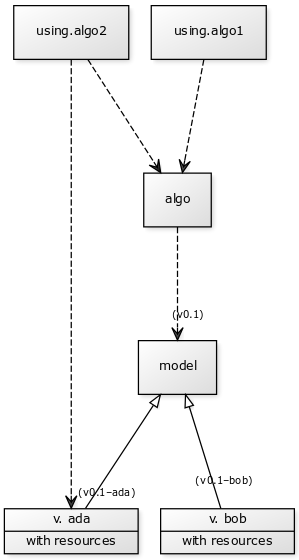
\includegraphics[width=200pt]{res/packaging_version_B.png}
\caption{Packaging Version B}
\label{fig:pkgsysB}
\end{figure}


\subsubsection{Version C}

The third version we studied is the most simple one: as illustrated on Figure \ref{fig:pkgsysC}, instead of splitting everything in separate package, only annotators are packaged independently of pipelines and resources, which are grouped together. On the one hand this system couldn't be simpler but on the other, since pipelines often involve several engine annotators that are themselves used in several pipelines, the coupling of models and the corresponding algorithm implies that many packages have to be created to support each combination of models.


\begin{figure}
\centering
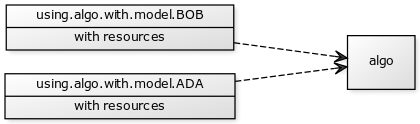
\includegraphics[width=200pt]{res/packaging_version_C.png}
\caption{Packaging Version C}
\label{fig:pkgsysC}
\end{figure}

\subsubsection{The verdict - Version D}

After exploring possibilities offered by the Maven packaging system we analysed how resources and engines are related to each others and used by pipelines in bluima. Figure \ref{fig:pkgsysD} depicts those relations. It was also considered that repackaging is an acceptable cost to swap models. The most important point was avoiding at all cost to package an exponentially huge number of pipelines to match each and every possible combinations and for this reason version C was discarded.

We also reflected on the structure of the algorithm, especially on their input arguments. We came to the conclusion that, mostly for flexibility, they should accept \ID{InputStream}s as input and not be bound to any models. Instead, the pipelines will be in charge to give them the proper resource data streams. Therefore the pipeline will have dependencies toward algorithms and models.

Finally, in order to centralise code and simplify loading resources we introduce \ID{ModelProxy}, a utility class used by pipelines that, given a \ID{String} representing a class name, opens a stream to a given file inside the class' jar archive.

In some cases, when processing the resource as a stream, it can be convenient to have access to its original filename (e.g. when reading a compressed archive). Therefore we encapsulate the name and the stream in a class -- \ID{ModelStream} -- that can be seen as a specialised \ID{InputStream} with a filename property.

\begin{figure}
\centering
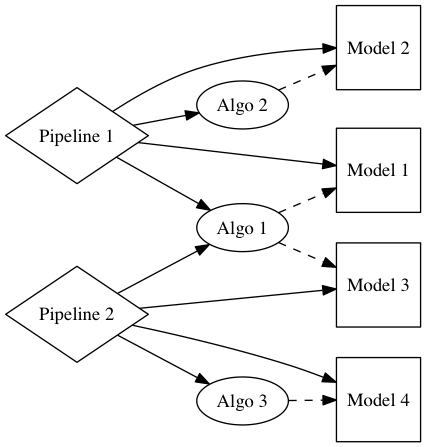
\includegraphics[width=200pt]{res/packaging_version_D.png}
\caption{Packaging Version D}
\label{fig:pkgsysD}
\end{figure}


\subsection{Restructuring bluima}
\label{sec:restructuring_bluima}

\TODO{better explain strategy before details}

Now that the packaging strategy for annotators and their resources has been designed we can actually apply it. It was decided to start with a relatively easy annotator -- namely \ID{SentenceAnnotator} which is part of OpenNLP -- to make sure our previous decision was indeed viable. The approach was based on an iterative process that can be applied to other modules as well. However, let's first take a step back and discuss the file hierarchy and how the different modules are related to each others.

\subsubsection{File Hierarchy}

We wanted to create a structured, yet flexible, file hierarchy for the annotators and their
resources. Since we are using Maven, we based our design on parent-child relationship in the
\ID{pom.xml} files: the root pom file, in addition to actually loading its children, defines the
main settings, such as the Java version to use or the list of general dependencies, that will be
shared with every of its children. The root pom file references both modules \PATH{modules/pom.xml}
and \PATH{resources/pom.xml} that are responsible for loading their own children, that is the different annotators or utilities for the former and the actual resource for the latter.

It follows that when running the install (or test) command on the root Maven project then every algorithms and resources are installed (or tested).

\subsubsection{Case Study: Converting OpenNLP}

When converting an annotator such as \ID{SentenceAnnotator}, the first thing to do is to identify the unit test responsible for its quality \TODO{add details on unit test in §bluima/§sherlok}. In this case, the annotator was imported from UIMA \TODO{ref} and it was still based on the XML engine descriptor \TODO{ref} \TODO{add explanation/contrast between XML engine descriptor \& java code in §bluima}. Therefore, we first have to make it compatible with the new and compact pipeline runner from uimaFIT \TODO{ref}.

Once the unit tests are properly working, we move on to the generation of the resource packages. Since this phase is completely repetitive, we devised a script \TODO{ref to wiki} to make the developer live less cumbersome: given a resource file, a resource name and a few other technical details we can produce a resource package, as described previously, that is ready to be used with an annotator.

However, many annotators are currently using Java \ID{File} parameters, or Java \ID{String}s pointing to a local file. Therefore, we have to refactor these annotators and their dependencies in order to use \ID{ModelStream} instead. The following strategy was applied to convert PoS, Token and Chunk annotator of OpenNLP:

\begin{enumerate}

\item Renaming the \ID{PARAM\_MODEL\_FILE} parameter (or any similar properties) of the annotator into \ID{PARAM\_MODEL}.

\item Updating its \ID{initialize} method to load a \ID{ModelStream} through \ID{ModelProxy} and the \ID{PARAM\_MODEL} parameter.

\item Updating the annotator's dependencies such that they can be constructed from \ID{ModelStream}. Usually this plays well with the current implementation that must at some point use a \ID{FileInputStream}. Hence, we can plug in our custom stream in place of the regular \ID{FileInputStream} without restructuring the dependencies too much.

\item Updating the dependency list in the annotator's \ID{pom.xml} file to reflect any additional resource dependency.

\end{enumerate}

Finally, at this last point the unit test should be updated to use resource package instead of
absolute path to the resource file with \ID{PARAM\_MODEL}.

\subsection{Pipeline Configuration in Sherlok}

\TODO{explain how this gets configured in Sherlok}


\section{Future Work}

\TODO{ideas? support for more variable url pattern (svn, ...) }
\TODO{overview figure, e.g.  Sherlok's Linnaeus bundle, that downloads the bluima Maven jar (that itself depends on the Linnaeus Maven library) and the Linnaeus config file; Sherlok's Linnaeus pipeline that uses them to annotate species}

\TODO{text extractor}

%provided that there is an adaptor to extract the actual text, and pull out the interesting metadata
%for the user. Text adaptors can extract more than just the raw text. For example, a PDF extractor
%could include information about text emphasis, whether a word is part of a section title, if proper
%name is an author or replace images by a text description.

\begin{thebibliography}{99}

\bibitem{bbp}
    Blue Brain Project,
    \href{http://bluebrain.epfl.ch/}{bluebrain.epfl.ch}

\bibitem{sherlok}
    Sherlok,
    \href{http://sherlok.io}{sherlok.io}

\bibitem{bluima}
    Bluima,
	\TODO{paper},
    \href{https://github.com/BlueBrain/bluima}{github.com/BlueBrain/bluima}

\bibitem{bluima_2013}
    Bluima: a UIMA-based NLP Toolkit for Neuroscience,
    by R. Richardet,
    Proceedings of the 3rd Workshop on Unstructured Information Management Architecture, Darmstadt,
    Germany, 2013, pp. 34–41, Gesellschaft für Sprachtechnologie und Computerlinguistik.

\bibitem{uima}
    Apache UIMA,
	\TODO{paper},
    \href{https://uima.apache.org/}{uima.apache.org}

\bibitem{uimafit}
    Apache uimaFIT,
    \href{https://uima.apache.org/uimafit.html}{uima.apache.org/uimafit.html}

\bibitem{cas}
    Design and implementation of the UIMA Common Analysis System,
    by T. Götz and O. Suhre,
    IBM SYSTEMS JOURNAL, VOL 43, NO 3, 2004

\bibitem{ruta}
    Apache RUTA,
	\TODO{paper},
    \href{https://uima.apache.org/ruta.html}{uima.apache.org/ruta.html}

\bibitem{maven}
    Apache Maven,
    \href{https://maven.apache.org/}{maven.apache.org}

\bibitem{apachefundation}
    The Apache Software Foundation,
    \href{http://www.apache.org/}{www.apache.org}

\bibitem{opennlp}
    Apache OpenNLP,
    \href{https://opennlp.apache.org/}{opennlp.apache.org}

\bibitem{linnaeus}
    Linnaeus,
	\TODO{paper},
    \href{http://linnaeus.sourceforge.net/}{linnaeus.sourceforge.net}

\bibitem{genia}
    GENIA corpus,
	\TODO{paper},
    \href{http://www.nactem.ac.uk/aNT/genia.html}{www.nactem.ac.uk/aNT/genia.html}


\end{thebibliography}

%\begin{appendix}
%  \listoffigures
%  \listoftables
%  \lstlistoflistings
%\end{appendix}

\end{document}
